% Options for packages loaded elsewhere
% Options for packages loaded elsewhere
\PassOptionsToPackage{unicode}{hyperref}
\PassOptionsToPackage{hyphens}{url}
%
\documentclass[
  ignorenonframetext,
  aspectratio=169,
  handout]{beamer}
\newif\ifbibliography
\usepackage{pgfpages}
\setbeamertemplate{caption}[numbered]
\setbeamertemplate{caption label separator}{: }
\setbeamercolor{caption name}{fg=normal text.fg}
\beamertemplatenavigationsymbolsempty
% remove section numbering
\setbeamertemplate{part page}{
  \centering
  \begin{beamercolorbox}[sep=16pt,center]{part title}
    \usebeamerfont{part title}\insertpart\par
  \end{beamercolorbox}
}
\setbeamertemplate{section page}{
  \centering
  \begin{beamercolorbox}[sep=12pt,center]{section title}
    \usebeamerfont{section title}\insertsection\par
  \end{beamercolorbox}
}
\setbeamertemplate{subsection page}{
  \centering
  \begin{beamercolorbox}[sep=8pt,center]{subsection title}
    \usebeamerfont{subsection title}\insertsubsection\par
  \end{beamercolorbox}
}
% Prevent slide breaks in the middle of a paragraph
\widowpenalties 1 10000
\raggedbottom
\AtBeginPart{
  \frame{\partpage}
}
\AtBeginSection{
  \ifbibliography
  \else
    \frame{\sectionpage}
  \fi
}
\AtBeginSubsection{
  \frame{\subsectionpage}
}
\usepackage{iftex}
\ifPDFTeX
  \usepackage[T1]{fontenc}
  \usepackage[utf8]{inputenc}
  \usepackage{textcomp} % provide euro and other symbols
\else % if luatex or xetex
  \usepackage{unicode-math} % this also loads fontspec
  \defaultfontfeatures{Scale=MatchLowercase}
  \defaultfontfeatures[\rmfamily]{Ligatures=TeX,Scale=1}
\fi
\usepackage{lmodern}

\ifPDFTeX\else
  % xetex/luatex font selection
\fi
% Use upquote if available, for straight quotes in verbatim environments
\IfFileExists{upquote.sty}{\usepackage{upquote}}{}
\IfFileExists{microtype.sty}{% use microtype if available
  \usepackage[]{microtype}
  \UseMicrotypeSet[protrusion]{basicmath} % disable protrusion for tt fonts
}{}
\makeatletter
\@ifundefined{KOMAClassName}{% if non-KOMA class
  \IfFileExists{parskip.sty}{%
    \usepackage{parskip}
  }{% else
    \setlength{\parindent}{0pt}
    \setlength{\parskip}{6pt plus 2pt minus 1pt}}
}{% if KOMA class
  \KOMAoptions{parskip=half}}
\makeatother


\usepackage{longtable,booktabs,array}
\newcounter{none} % for unnumbered tables
\usepackage{calc} % for calculating minipage widths
\usepackage{caption}
% Make caption package work with longtable
\makeatletter
\def\fnum@table{\tablename~\thetable}
\makeatother
\usepackage{graphicx}
\makeatletter
\newsavebox\pandoc@box
\newcommand*\pandocbounded[1]{% scales image to fit in text height/width
  \sbox\pandoc@box{#1}%
  \Gscale@div\@tempa{\textheight}{\dimexpr\ht\pandoc@box+\dp\pandoc@box\relax}%
  \Gscale@div\@tempb{\linewidth}{\wd\pandoc@box}%
  \ifdim\@tempb\p@<\@tempa\p@\let\@tempa\@tempb\fi% select the smaller of both
  \ifdim\@tempa\p@<\p@\scalebox{\@tempa}{\usebox\pandoc@box}%
  \else\usebox{\pandoc@box}%
  \fi%
}
% Set default figure placement to htbp
\def\fps@figure{htbp}
\makeatother





\setlength{\emergencystretch}{3em} % prevent overfull lines

\providecommand{\tightlist}{%
  \setlength{\itemsep}{0pt}\setlength{\parskip}{0pt}}



 


\makeatletter
\@ifpackageloaded{caption}{}{\usepackage{caption}}
\AtBeginDocument{%
\ifdefined\contentsname
  \renewcommand*\contentsname{Table of contents}
\else
  \newcommand\contentsname{Table of contents}
\fi
\ifdefined\listfigurename
  \renewcommand*\listfigurename{List of Figures}
\else
  \newcommand\listfigurename{List of Figures}
\fi
\ifdefined\listtablename
  \renewcommand*\listtablename{List of Tables}
\else
  \newcommand\listtablename{List of Tables}
\fi
\ifdefined\figurename
  \renewcommand*\figurename{Figure}
\else
  \newcommand\figurename{Figure}
\fi
\ifdefined\tablename
  \renewcommand*\tablename{Table}
\else
  \newcommand\tablename{Table}
\fi
}
\@ifpackageloaded{float}{}{\usepackage{float}}
\floatstyle{ruled}
\@ifundefined{c@chapter}{\newfloat{codelisting}{h}{lop}}{\newfloat{codelisting}{h}{lop}[chapter]}
\floatname{codelisting}{Listing}
\newcommand*\listoflistings{\listof{codelisting}{List of Listings}}
\makeatother
\makeatletter
\makeatother
\makeatletter
\@ifpackageloaded{caption}{}{\usepackage{caption}}
\@ifpackageloaded{subcaption}{}{\usepackage{subcaption}}
\makeatother

\usepackage{bookmark}
\IfFileExists{xurl.sty}{\usepackage{xurl}}{} % add URL line breaks if available
\urlstyle{same}
\hypersetup{
  pdftitle={Molecular Degrees of Freedom},
  pdfauthor={Davit Potoyan},
  hidelinks,
  pdfcreator={LaTeX via pandoc}}


\title{\texorpdfstring{Molecular Degrees of
Freedom}{Molecular Degrees of Freedom}}
\subtitle{\texorpdfstring{Chem 3240 · Lecture
4.1}{Chem 3240 · Lecture 4.1}}
\author{Davit Potoyan}
\date{}

\begin{document}
\frame{\titlepage}


\begin{frame}
\begin{block}{Where we are headed}
\protect\phantomsection\label{where-we-are-headed}
Bound systems have \textbf{quantized} energy.

Next: how each kind of motion is quantized, and how
\textbf{spectroscopy} probes it.

Toy models map onto real motions:

\begin{itemize}
\tightlist
\item
  \textbf{Particle in a box} → translation
\item
  \textbf{Harmonic oscillator} → vibration
\item
  \textbf{Rigid rotor} → rotation
\end{itemize}
\end{block}

\begin{block}{Four kinds of molecular motion}
\protect\phantomsection\label{four-kinds-of-molecular-motion}
\begin{columns}[T]
\begin{column}{0.5\linewidth}
\pandocbounded{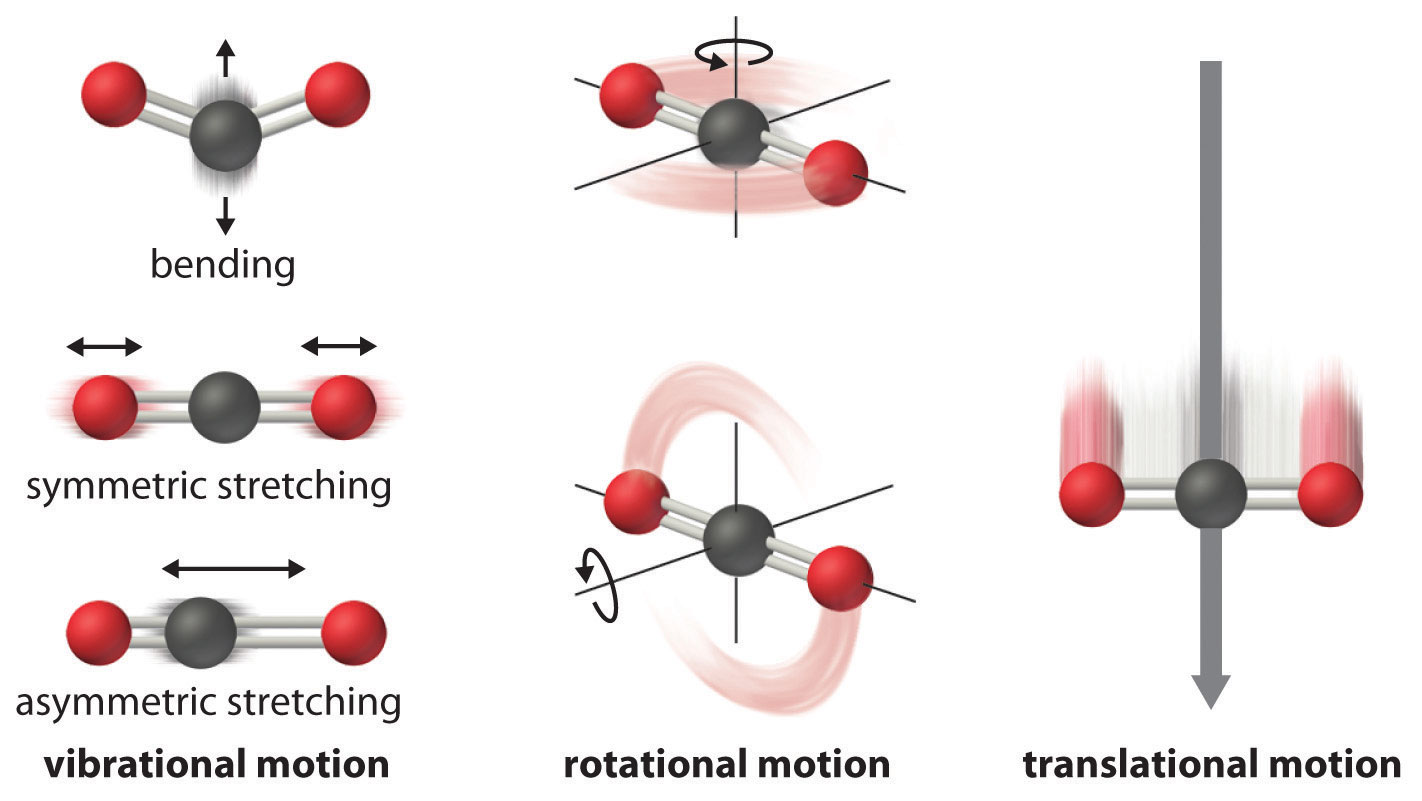
\includegraphics[keepaspectratio]{../../ch04/images/mol-DOF.jpg}}
\end{column}

\begin{column}{0.5\linewidth}
A molecule's energy splits into independent pieces:

\[E = \epsilon_{trans} + \epsilon_{rot} + \epsilon_{vib} + \epsilon_{elec}\]

Each kind of motion is \textbf{quantized differently}.
\end{column}
\end{columns}
\end{block}

\begin{block}{Different spacings, different spectroscopy}
\protect\phantomsection\label{different-spacings-different-spectroscopy}
\begin{columns}[T]
\begin{column}{0.45\linewidth}
\pandocbounded{\includegraphics[keepaspectratio]{../../ch04/images/Levels1.gif}}
\end{column}

\begin{column}{0.55\linewidth}
Boundary conditions set the \textbf{level spacing}.

Electronic ≫ vibrational ≫ rotational ≫ translational.

Each scale → its \textbf{own spectroscopy}.
\end{column}
\end{columns}
\end{block}

\begin{block}{Counting: 3N nuclear coordinates}
\protect\phantomsection\label{counting-3n-nuclear-coordinates}
\begin{columns}[T]
\begin{column}{0.5\linewidth}
\pandocbounded{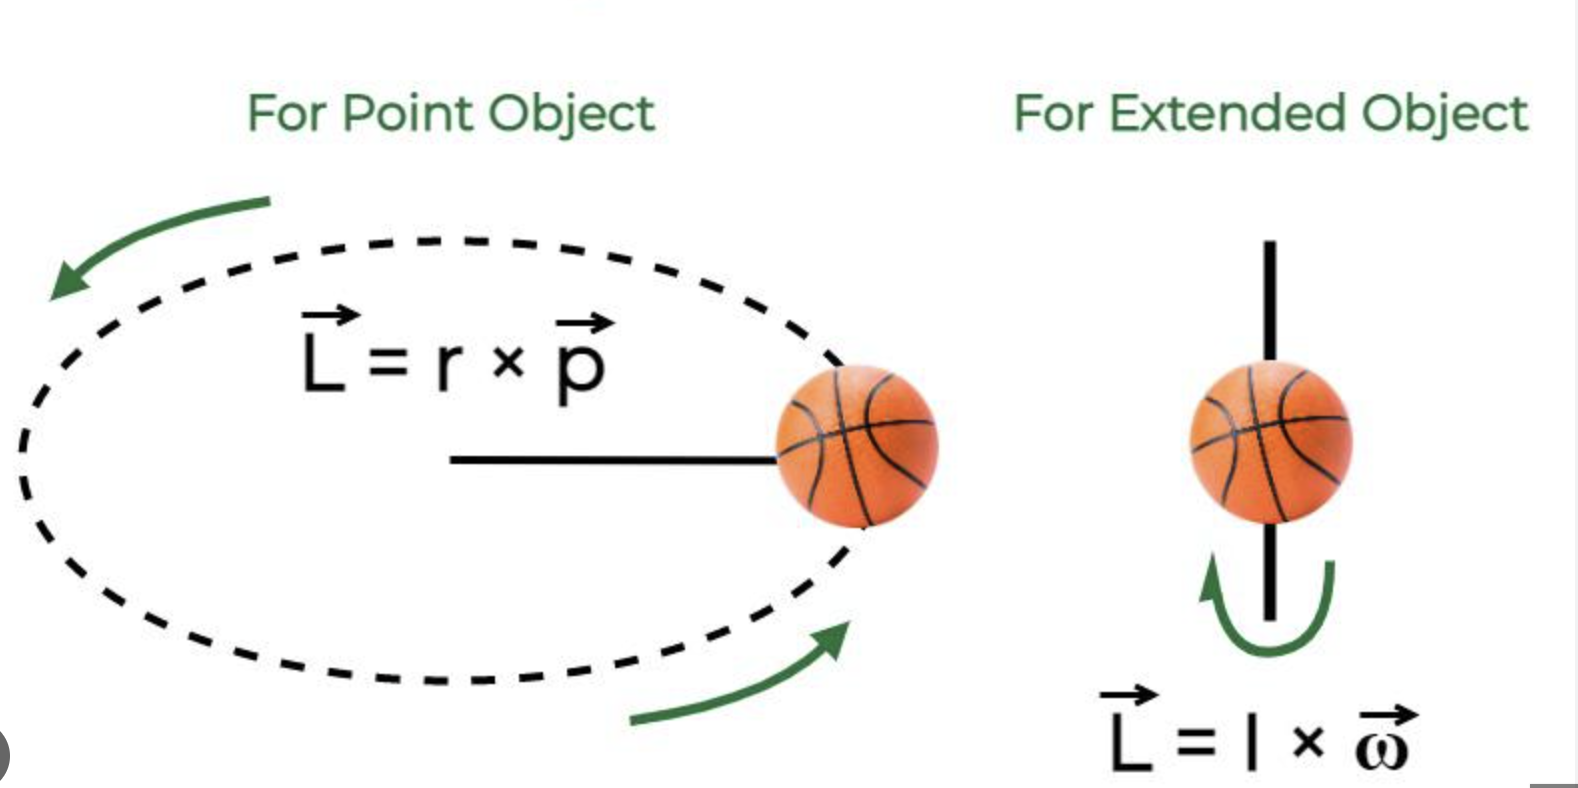
\includegraphics[keepaspectratio]{../../ch04/images/point_extended.png}}
\end{column}

\begin{column}{0.5\linewidth}
\(N\) nuclei, each with \(x, y, z\):

\[3N \text{ total degrees of freedom}\]

\textbf{Born--Oppenheimer}: separate nuclei from electrons.

\[\hat{H} = \sum_{i=1}^{N} -\frac{\hbar^2}{2m_i}\nabla_{R_i}^2 + E(R_1,\dots,R_N)\]
\end{column}
\end{columns}
\end{block}

\begin{block}{Splitting the Hamiltonian}
\protect\phantomsection\label{splitting-the-hamiltonian}
The nuclear motion separates into three parts:

\[\hat{H} = \hat{H}_{tr} + \hat{H}_{rot} + \hat{H}_{vib}\]

\begin{itemize}
\tightlist
\item
  \(\hat{H}_{tr}\), \(\hat{H}_{rot}\): \textbf{no potential}
\item
  \(\hat{H}_{vib}\): carries the potential \(E\) between nuclei
\end{itemize}

Separation lets the wavefunction \textbf{factorize}:

\[\psi = \psi_{tr}\,\psi_{rot}\,\psi_{vib}\]
\end{block}

\begin{block}{Three Schrödinger equations}
\protect\phantomsection\label{three-schruxf6dinger-equations}
\[\hat{H}_{tr}\psi_{tr} = E_{tr}\psi_{tr}\]

\[\hat{H}_{rot}\psi_{rot} = E_{rot}\psi_{rot}\]

\[\hat{H}_{vib}\psi_{vib} = E_{vib}\psi_{vib}\]

\textbf{Translation}: no boundary condition → continuous spectrum.

\textbf{Rotation} (cyclic boundary) and \textbf{vibration} (potential
\(E\)) → \textbf{quantized}.
\end{block}

\begin{block}{Bookkeeping the degrees of freedom}
\protect\phantomsection\label{bookkeeping-the-degrees-of-freedom}
Start with \(3N\), then subtract:

\begin{itemize}
\tightlist
\item
  \textbf{Translation}: always \(3\) → leaves \(3N - 3\)
\end{itemize}

\begin{itemize}
\tightlist
\item
  \textbf{Rotation}: \(3\) nonlinear, \(2\) linear
\end{itemize}

\begin{itemize}
\tightlist
\item
  \textbf{Vibration}: whatever remains

  \begin{itemize}
  \tightlist
  \item
    Nonlinear: \(3N - 6\)
  \item
    Linear: \(3N - 5\)
  \end{itemize}
\end{itemize}
\end{block}

\begin{block}{At a glance}
\protect\phantomsection\label{at-a-glance}
{\def\LTcaptype{none} % do not increment counter
\begin{longtable}[]{@{}lccc@{}}
\toprule\noalign{}
& Translation & Rotation & Vibration \\
\midrule\noalign{}
\endhead
\textbf{Linear} & 3 & 2 & \(3N-5\) \\
\textbf{Nonlinear} & 3 & 3 & \(3N-6\) \\
\bottomrule\noalign{}
\end{longtable}
}

Linear molecules have \textbf{one fewer} rotation, so \textbf{one more}
vibration.
\end{block}
\end{frame}

\begin{frame}{Takeaway}
\protect\phantomsection\label{takeaway}
\begin{quote}
A molecule has \(3N\) degrees of freedom: \(3\) translation, \(2\) or
\(3\) rotation, the rest (\(3N-5\) or \(3N-6\)) vibration.
Born--Oppenheimer separation factorizes the motion, and boundary
conditions decide which parts are quantized and how spectroscopy probes
them.
\end{quote}
\end{frame}




\end{document}
